\chapter{RESULTS AND DISCUSSION}
\label{chap:results}

This chapter presents the results in the same sequence as the methodology in
Chapter~\ref{chap:methodology}. Sensor validation is discussed first because
the protection decisions depend on calibrated voltage, current, and
temperature measurements. The following sections then interpret overload
protection, socket-heating characterization, socket-heating protection
validation, series arc-fault detection, TinyML model performance, and the
overall feasibility of the prototype.

\section{Sensor Validation}
\label{sec:ch4-sensor-validation}

The sensor-validation results determine whether the calibrated measurements
were reliable enough for the protection decisions described in
Chapter~\ref{chap:methodology}. In this section, the voltage, current, and
device-temperature channels are interpreted in terms of decision reliability rather
than as isolated measurement exercises.

\subsection{Voltage Sensor Validation}
\label{sec:ch4-voltage-validation}

The voltage sensor was compared with a Fluke 115 True RMS multimeter at ten
test points.
\begin{table}[H]
  \centering
  \caption{Validation results for the voltage sensor}
  \label{tab:ch4-voltage-validation}
  \begin{tabular}{ccccc}
    \toprule
    \textbf{Test} & \textbf{Device (V)} & \textbf{Fluke (V)} & \textbf{Abs. error (V)} & \textbf{Squared error (V$^2$)} \\
    \midrule
    1 & 181.0 & 184.7 & 3.7 & 13.69 \\
    2 & 196.1 & 192.8 & 3.3 & 10.89 \\
    3 & 198.4 & 201.9 & 3.5 & 12.25 \\
    4 & 210.3 & 213.6 & 3.3 & 10.89 \\
    5 & 223.8 & 219.7 & 4.1 & 16.81 \\
    6 & 221.0 & 225.4 & 4.4 & 19.36 \\
    7 & 234.6 & 230.9 & 3.7 & 13.69 \\
    8 & 232.7 & 236.5 & 3.8 & 14.44 \\
    9 & 247.5 & 243.1 & 4.4 & 19.36 \\
    10 & 244.3 & 249.2 & 4.9 & 24.01 \\
    \bottomrule
  \end{tabular}
\end{table}

Table~\ref{tab:ch4-voltage-validation} shows the validation results for the voltage sensor. 
The corrected prototype readings produced an MAE of 3.910V, MSE
of 15.539V$^2$, and RMSE of 3.94V. These errors are small relative to the
firmware voltage bands in Table~\ref{tab:ch3-voltage-thresholds}; therefore,
the calibrated voltage channel is adequate for distinguishing normal operation
from the undervoltage and overvoltage regions used in this prototype.
The result supports voltage
state discrimination, but it does not by itself certify the device for
utility-grade metering.

\subsection{Current Sensor Validation}
\label{sec:ch4-current-validation}

The current sensor was compared with an Ingco clamp meter.
\begin{table}[H]
  \centering
  \caption{Validation results for the current sensor}
  \label{tab:ch4-current-validation}
  \begin{tabular}{ccccc}
    \toprule
    \textbf{Test} & \textbf{Device (A)} & \textbf{Clamp meter (A)} & \textbf{Abs. error (A)} & \textbf{Squared error (A$^2$)} \\
    \midrule
    1 & 0.66 & 0.68 & 0.02 & 0.0004 \\
    2 & 1.98 & 1.94 & 0.04 & 0.0016 \\
    3 & 5.00 & 5.11 & 0.11 & 0.0121 \\
    4 & 7.80 & 7.63 & 0.17 & 0.0289 \\
    5 & 8.97 & 9.14 & 0.17 & 0.0289 \\
    6 & 10.76 & 10.58 & 0.18 & 0.0324 \\
    7 & 11.84 & 12.06 & 0.22 & 0.0484 \\
    8 & 14.00 & 13.74 & 0.26 & 0.0676 \\
    9 & 14.34 & 14.67 & 0.33 & 0.1089 \\
    10 & 16.14 & 15.86 & 0.28 & 0.0784 \\
    \bottomrule
  \end{tabular}
\end{table}

Table~\ref{tab:ch4-current-validation} shows that error increased slightly at
higher currents but remained much smaller than the distance between the warning
and sustained-trip thresholds.
The current channel
produced an MAE of 0.178A, MSE of 0.04076A$^2$, and RMSE of 0.202A. This
level of error is acceptable for the implemented warning and sustained-trip
thresholds because the warning threshold is 10.0A and the sustained-overload
threshold is 14.5A. The same current channel is also used by the socket
thermal model and the TinyML feature extractor, so a low RMS-current error
improves both threshold and feature reliability.
This supports the overload results discussed in
Section~\ref{sec:ch4-overload-protection}.

\subsection{Device Temperature Measurement Validation}
\label{sec:ch4-temperature-validation}

The TTC05103JSY 10k$\Omega$ thermistor was compared with a reference infrared
thermometer at the sensor measurement point.
\begin{table}[H]
  \centering
  \caption{Validation results for the device temperature measurement thermistor channel}
  \label{tab:ch4-temperature-validation}
  \begin{tabular}{ccccc}
    \toprule
    \textbf{Test} & \textbf{Device ($^\circ$C)} & \textbf{IR thermometer ($^\circ$C)} & \textbf{Abs. error ($^\circ$C)} & \textbf{Squared error ($^\circ$C$^2$)} \\
    \midrule
    1 & 27.9 & 27.4 & 0.5 & 0.25 \\
    2 & 31.1 & 31.8 & 0.7 & 0.49 \\
    3 & 37.7 & 36.6 & 1.1 & 1.21 \\
    4 & 41.1 & 41.9 & 0.8 & 0.64 \\
    5 & 48.2 & 47.3 & 0.9 & 0.81 \\
    6 & 51.2 & 52.5 & 1.3 & 1.69 \\
    7 & 59.0 & 58.1 & 0.9 & 0.81 \\
    8 & 61.6 & 63.2 & 1.6 & 2.56 \\
    9 & 67.8 & 66.8 & 1.0 & 1.00 \\
    10 & 68.3 & 69.7 & 1.4 & 1.96 \\
    \bottomrule
  \end{tabular}
\end{table}

Table~\ref{tab:ch4-temperature-validation} supports the use of the thermistor channel as a
stable observable input for the thermal estimator. The device temperature measurement channel produced an MAE
of 1.02°C, MSE of 1.142°C$^2$, and RMSE of 1.07°C. This
validates the thermistor channel itself, but it must not be interpreted as a
direct validation of internal contact temperature. 
Hence, it reinforces the
methodological need for the compensated socket-temperature model because the
sensor is external to the highest-temperature contact interface.
The heating tests later
show that the socket terminal can be much hotter than the external thermistor reading
or compensated estimate. 

\section{Overload Protection}
\label{sec:ch4-overload-protection}

Five overload-related trials were conducted using high-power load combinations.
All trials entered the overload-warning region, but only the most severe case
remained above the sustained-overload criterion long enough to trip the relay.
This matches the firmware method in Section~\ref{sec:ch3-overload-protection},
where warning and sustained trip are intentionally separated.

Table~\ref{tab:ch4-overload-evaluation} summarizes the overload results.
\begin{table}[H]
  \centering
  \caption{Overload evaluation results}
  \label{tab:ch4-overload-evaluation}
  \small
  \begin{tabular}{p{0.06\textwidth}p{0.30\textwidth}p{0.09\textwidth}p{0.09\textwidth}p{0.08\textwidth}p{0.10\textwidth}p{0.12\textwidth}}
    \toprule
    Trial & Load setup & Mean V & Mean A & Peak A & Warning & Trip latency \\
    \midrule
    1 & 1300W electric kettle + water heater & 231.8 & 12.87 & 14.85 & Yes & -- \\
    2 & 1300W electric kettle + 1500W electric kettle & 229.5 & 12.33 & 13.63 & Yes & -- \\
    3 & 1500W electric kettle + water heater & 229.6 & 13.36 & 14.86 & Yes & -- \\
    4 & 1300W electric kettle + water heater + 2 $\times$ 500W halogen lamp & 224.0 & 17.30 & 19.73 & Yes & 61.3s \\
    5 & 1300W electric kettle + water heater + 500W halogen lamp & 229.1 & 14.42 & 16.23 & Yes & -- \\
    \bottomrule
  \end{tabular}
\end{table}

Table~\ref{tab:ch4-overload-evaluation} shows that warning occurred in all
heavy-load cases, while relay disconnection occurred only in Trial 4. The mean
current of Trial 4 was 17.30A, clearly above the 14.5A sustained-overload
threshold, and the 61.3s trip latency agrees with the intended 60s
persistence behavior. Trials 1, 3, and 5 reached peak values near or above the
sustained threshold, but they did not remain in the sustained-overload state
long enough for the score to reach the trip value.

This result supports the overload objective because the prototype behaved as a
warning-and-persistence device rather than an instantaneous current cutoff. The
main limitation is that the tests were conducted with selected laboratory load
combinations; broader appliance combinations and longer-duration thermal tests
would be needed before choosing final consumer-product trip curves.

\section{Socket-Heating Characterization}
\label{sec:ch4-socket-heating-characterization}

The socket-heating characterization compared a normal socket with a degraded
socket under similar current levels. The purpose was to verify the Chapter 3
assumption that socket temperature is not determined by current alone; contact
condition changes the rate and final magnitude of heating.
The plotted trends in this section were generated from the full
characterization records in Appendix~\ref{app:c}.

The water-heater-only characterization trend is shown in
Figure~\ref{fig:ch4-char-water-heater}.
\begin{figure}[H]
  \centering
  \socketCharPlot{1}{240}
  \caption{Water heater temperature trend during socket-heating characterization.}
  \label{fig:ch4-char-water-heater}
\end{figure}

Figure~\ref{fig:ch4-char-water-heater} shows that at about 5.2A, both socket
conditions stayed below the 38.2°C comparison point within the 240min
window. The corroded socket still ended hotter than the normal socket, showing
the beginning of contact-condition influence even at the lowest tested load.

The water heater plus one halogen lamp trend is shown in
Figure~\ref{fig:ch4-char-one-lamp}.
\begin{figure}[H]
  \centering
  \socketCharPlot{2}{240}
  \caption{Water heater plus one halogen lamp temperature trend during characterization.}
  \label{fig:ch4-char-one-lamp}
\end{figure}

Figure~\ref{fig:ch4-char-one-lamp} shows clearer separation between normal and
corroded behavior. The corroded socket reached the 38.2°C comparison
point, while the normal socket did not reach that point within the same window.

The water heater plus two halogen lamps trend is shown in
Figure~\ref{fig:ch4-char-two-lamps}.
\begin{figure}[H]
  \centering
  \socketCharPlot{3}{240}
  \caption{Water heater plus two halogen lamps temperature trend during characterization.}
  \label{fig:ch4-char-two-lamps}
\end{figure}

Figure~\ref{fig:ch4-char-two-lamps} shows that the degraded socket reached the
comparison temperature much earlier than the normal socket. The terminal
temperature also rose above the NTC temperature, supporting the need to treat
the external NTC as an under-reading proxy rather than the actual hotspot.

The water heater plus three halogen lamps trend is shown in
Figure~\ref{fig:ch4-char-three-lamps}.
\begin{figure}[H]
  \centering
  \socketCharPlot{4}{240}
  \caption{Water heater plus three halogen lamps temperature trend during characterization.}
  \label{fig:ch4-char-three-lamps}
\end{figure}

Figure~\ref{fig:ch4-char-three-lamps} shows the strongest time-to-threshold
contrast in the characterization set: the corroded socket reached the
comparison point after only 7min, while the normal socket reached it after
52min.

The water heater plus four halogen lamps trend is shown in
Figure~\ref{fig:ch4-char-four-lamps}.
\begin{figure}[H]
  \centering
  \socketCharPlot{5}{195}
  \caption{Water heater plus four halogen lamps temperature trend during characterization.}
  \label{fig:ch4-char-four-lamps}
\end{figure}

Figure~\ref{fig:ch4-char-four-lamps} shows that the high-current degraded
trial developed rapidly and was stopped after a short observation window. The
terminal temperature reached 45.8°C within 4min even though the final
NTC reading was only 36.9°C.

Table~\ref{tab:ch4-heating-characterization} summarizes the characterization
data used to interpret these trends.
\begin{table}[H]
  \centering
  \caption{Summary of socket-heating characterization data}
  \label{tab:ch4-heating-characterization}
  \small
  \setlength{\tabcolsep}{2pt}
  \begin{tabular*}{\textwidth}{@{\extracolsep{\fill}}p{0.22\textwidth}p{0.105\textwidth}p{0.13\textwidth}p{0.08\textwidth}p{0.11\textwidth}p{0.135\textwidth}p{0.09\textwidth}@{}}
    \toprule
    Load case & Socket & Time to 38.2°C & Mean A & Final NTC & Final terminal & Window (min) \\
    \midrule
    Water heater & Normal & -- & 5.18 & 33.9 & 31.5 & 240 \\
    Water heater & Corroded & -- & 5.16 & 35.6 & 37.4 & 240 \\
    Water heater + 1 lamp & Normal & -- & 7.12 & 37.7 & 37.6 & 240 \\
    Water heater + 1 lamp & Corroded & 95 & 7.10 & 40.4 & 43.2 & 240 \\
    Water heater + 2 lamps & Normal & 105 & 9.07 & 40.2 & 40.8 & 240 \\
    Water heater + 2 lamps & Corroded & 48 & 9.05 & 41.0 & 44.5 & 120 \\
    Water heater + 3 lamps & Normal & 52 & 11.06 & 43.2 & 45.8 & 240 \\
    Water heater + 3 lamps & Corroded & 7 & 11.15 & 38.8 & 53.0 & 8 \\
    Water heater + 4 lamps & Normal & 44 & 13.00 & 43.4 & 46.4 & 195 \\
    Water heater + 4 lamps & Corroded & -- & 13.10 & 36.9 & 45.8 & 4 \\
    \bottomrule
  \end{tabular*}
\end{table}

Table~\ref{tab:ch4-heating-characterization} confirms that degraded contact
changed both heating speed and hotspot severity. At about 9A, the corroded
socket reached 38.2°C in 48min compared with 105min for the normal
socket. At about 11A, the corroded socket reached the same point in 7min
compared with 52min for the normal socket. These results support the need for
the compensated thermal model described in Section~\ref{sec:ch3-socket-heating-models}.


\section{Socket-Heating Protection Validation}
\label{sec:ch4-socket-heating-protection}

Socket-heating protection validation evaluated the relay-facing estimated
socket temperature. The important distinction is between four temperatures:
the direct NTC temperature, the expected normal socket temperature, the
estimated socket temperature used by protection, and the reference terminal
temperature. The trip threshold applies to the estimated socket temperature,
while the reference terminal temperature shows how hot the socket contact area
became during the same trial.
The plotted trends in this section were generated from the full protection
validation records in Appendix~\ref{app:d}.

The water-heater-only protection trend is shown in
Figure~\ref{fig:ch4-protect-water-heater}.
\begin{figure}[H]
  \centering
  \socketProtectionPlot{1}{240}
  \caption{Water heater temperature trend during socket-heating protection validation.}
  \label{fig:ch4-protect-water-heater}
\end{figure}

Figure~\ref{fig:ch4-protect-water-heater} shows that the low-current case did
not trip for either socket condition within the observation window. The
corroded terminal still ended hotter than the normal terminal, but the
estimated socket temperature stayed below the 40°C trip threshold.

The water heater plus one halogen lamp protection trend is shown in
Figure~\ref{fig:ch4-protect-one-lamp}.
\begin{figure}[H]
  \centering
  \socketProtectionPlot{2}{240}
  \caption{Water heater plus one halogen lamp trend during protection validation.}
  \label{fig:ch4-protect-one-lamp}
\end{figure}

Figure~\ref{fig:ch4-protect-one-lamp} shows that the normal socket did not
trip, while the corroded socket reached a protection-relevant state after a
longer heating period. This supports the estimator's role in distinguishing
slow thermal buildup from immediate current overload.

The water heater plus two halogen lamps protection trend is shown in
Figure~\ref{fig:ch4-protect-two-lamps}.
\begin{figure}[H]
  \centering
  \socketProtectionPlot{3}{120}
  \caption{Water heater plus two halogen lamps trend during protection validation.}
  \label{fig:ch4-protect-two-lamps}
\end{figure}

Figure~\ref{fig:ch4-protect-two-lamps} shows that the corroded socket tripped
much earlier than the normal socket at approximately the same current. The
reference terminal temperature was already above the estimated value at trip,
which confirms that the estimator acts as an early proxy for a hotter internal
condition.

The water heater plus three halogen lamps protection trend is shown in
Figure~\ref{fig:ch4-protect-three-lamps}.
\begin{figure}[H]
  \centering
  \socketProtectionPlot{4}{58}
  \caption{Water heater plus three halogen lamps trend during protection validation.}
  \label{fig:ch4-protect-three-lamps}
\end{figure}

Figure~\ref{fig:ch4-protect-three-lamps} shows fast thermal development in
the corroded case. The relay acted within the short test window, while the
reference terminal temperature reached 55.0°C.

The water heater plus four halogen lamps protection trend is shown in
Figure~\ref{fig:ch4-protect-four-lamps}.
\begin{figure}[H]
  \centering
  \socketProtectionPlot{5}{46}
  \caption{Water heater plus four halogen lamps trend during protection validation.}
  \label{fig:ch4-protect-four-lamps}
\end{figure}

Figure~\ref{fig:ch4-protect-four-lamps} shows the most severe heating case.
The corroded socket tripped after 5min when the estimated socket temperature
reached 40.0°C, while the reference terminal temperature had already
reached 56.0°C.

Table~\ref{tab:ch4-heating-protection} summarizes the protection validation
results.
\begin{table}[H]
  \centering
  \caption{Socket-heating protection validation results}
  \label{tab:ch4-heating-protection}
  \small
  \setlength{\tabcolsep}{3pt}
  \begin{tabular}{@{}p{0.20\textwidth}p{0.10\textwidth}p{0.07\textwidth}p{0.09\textwidth}p{0.08\textwidth}p{0.10\textwidth}p{0.10\textwidth}p{0.07\textwidth}@{}}
    \toprule
    Load case & Socket & Mean A & NTC 38.2 & Est. 40 & Est. temp & Terminal & Relay \\
    \midrule
    Water heater & Normal & 5.17 & -- & -- & 32.7 & 33.8 & No \\
    Water heater & Corroded & 4.85 & -- & -- & 36.7 & 38.5 & No \\
    Water heater + 1 lamp & Normal & 7.11 & -- & -- & 38.1 & 40.3 & No \\
    Water heater + 1 lamp & Corroded & 7.10 & 100 & -- & 39.8 & 42.4 & Yes \\
    Water heater + 2 lamps & Normal & 9.06 & 100 & 120 & 40.0 & 43.2 & Yes \\
    Water heater + 2 lamps & Corroded & 9.04 & 48 & 52 & 40.0 & 44.1 & Yes \\
    Water heater + 3 lamps & Normal & 11.07 & 54 & -- & 39.9 & 43.9 & Yes \\
    Water heater + 3 lamps & Corroded & 11.14 & 7 & -- & 39.7 & 55.0 & Yes \\
    Water heater + 4 lamps & Normal & 13.02 & 44 & -- & 39.9 & 45.0 & Yes \\
    Water heater + 4 lamps & Corroded & 13.08 & 5 & 5 & 40.0 & 56.0 & Yes \\
    \bottomrule
  \end{tabular}
\end{table}

Table~\ref{tab:ch4-heating-protection} shows that degraded and higher-current
conditions tripped earlier than low-current or healthy-socket conditions. The
result supports the protection objective because the relay response followed
the compensated estimated socket temperature, not merely current magnitude. A
limitation remains: the external NTC and compensation model still
underestimated the hottest terminal temperature in severe degraded-contact
cases. The prototype therefore demonstrates useful complementary protection,
but a final certified design would need a validated thermal model across more
socket types, contact materials, enclosure conditions, and ambient conditions.


\section{Series Arc-Fault Detection}
\label{sec:ch4-series-arc-detection}

The series arc-fault tests evaluated whether waveform disturbance could be
converted into a relay decision. During arcing, the current waveform was
expected to show low-current gaps, restrike spikes, unstable cycle shape, and
changes in mid/high-frequency content. These behaviors correspond to the
features defined in Section~\ref{sec:ch3-waveform-features}, especially
maximum low-current run, low-current ratio, zero-dwell behavior, midband
residual ratio, and spectral flux.

The trial-level results are summarized as confusion matrices in
Table~\ref{tab:ch4-arc-confusion}. Here, ``relay trips'' is the positive
prototype response and ``arcing event'' is the positive ground-truth condition.
\begin{table}[H]
  \centering
  \caption{Trial-level confusion matrices for series arc-fault testing}
  \label{tab:ch4-arc-confusion}
  \begin{tabular}{p{0.26\textwidth}p{0.24\textwidth}cc}
    \toprule
    \textbf{Device group} & \textbf{Prototype response} & \textbf{Arcing event} & \textbf{Normal event} \\
    \midrule
    Recognized loads & Relay trips & 49 & 0 \\
    Recognized loads & Relay remains on & 1 & 50 \\
    \midrule
    Unrecognized loads & Relay trips & 47 & 1 \\
    Unrecognized loads & Relay remains on & 3 & 49 \\
    \midrule
    All tested loads & Relay trips & 96 & 1 \\
    All tested loads & Relay remains on & 4 & 99 \\
    \bottomrule
  \end{tabular}
\end{table}

Table~\ref{tab:ch4-arc-confusion} shows that the prototype detected 96 of 100
arc trials and produced one relay trip during 100 normal trials. The recognized
load group had no normal-event false trip and one missed arc event. The
unrecognized group was more difficult, with three missed arcs and one false
trip. This difference is expected because unrecognized devices introduce
waveform behavior not directly represented during model fitting.

The result supports the arc-detection objective under the tested laboratory
conditions. The classifier response was strongest when the arc created
persistent low-current gaps and spectral disturbance, allowing the leaky arc
counter to reach the relay-trip threshold. The missed trials indicate that not
all arcs produced equally strong or persistent feature responses, especially
when the load type differed from the fitted set. Therefore, the prototype
should be interpreted as a controlled feasibility demonstration, not as a
certified AFCI-equivalent device.

\section{Arc-Fault Dataset Summary}
\label{sec:ch4-arc-dataset-summary}

The cleaned arc-training dataset contained 49,296 rows, of which 283 were arc
markers, equivalent to about 0.577\% of the retained data. This confirms that
the problem was highly imbalanced: most frames represented normal operation
even in sessions that contained an arc event. The imbalance explains why
frame-level accuracy alone can be misleading; a classifier can appear accurate
by predicting mostly normal frames. Precision, recall, F1-score, and
event-level metrics are therefore needed to interpret the safety behavior.

Complete trial tables and raw collection logs are provided in
Appendices~\ref{app:e} and~\ref{app:f}. These appendices are important because
the summary table in the main text cannot show every feature frame, arc marker,
or relay-state transition.

\section{TinyML Model Performance}
\label{sec:ch4-tinyml-model-performance}

The TinyML results were interpreted at two levels. First, the embedded
prototype was evaluated by trial-level relay behavior in the laboratory.
Second, the exported Random Forest report was evaluated by held-out
frame-level and event-level metrics. Both views are useful: trial-level
behavior reflects the complete protection sequence, while frame-level metrics
show how the model performed before relay-counter persistence.

Table~\ref{tab:ch4-trial-metrics} gives the trial-level metrics for
recognized loads, unrecognized loads, and all loads combined.
\begin{table}[H]
  \centering
  \caption{Trial-level arc-fault performance metrics}
  \label{tab:ch4-trial-metrics}
  \begin{tabular}{lcccc}
    \toprule
    \textbf{Load group} & \textbf{Accuracy} & \textbf{Precision} & \textbf{Recall} & \textbf{F1-score} \\
    \midrule
    Recognized loads & 99.00\% & 100.00\% & 98.00\% & 98.99\% \\
    Unrecognized loads & 96.00\% & 97.92\% & 94.00\% & 95.92\% \\
    All tested loads & 97.50\% & 98.97\% & 96.00\% & 97.46\% \\
    \bottomrule
  \end{tabular}
\end{table}

Figure~\ref{fig:ch4-group-metrics} graphs the same four metrics by load
setup. This presentation compares like quantities across recognized,
unrecognized, and combined test groups; it does not mix unrelated metrics as
separate one-off bars.
\begin{figure}[H]
  \centering
  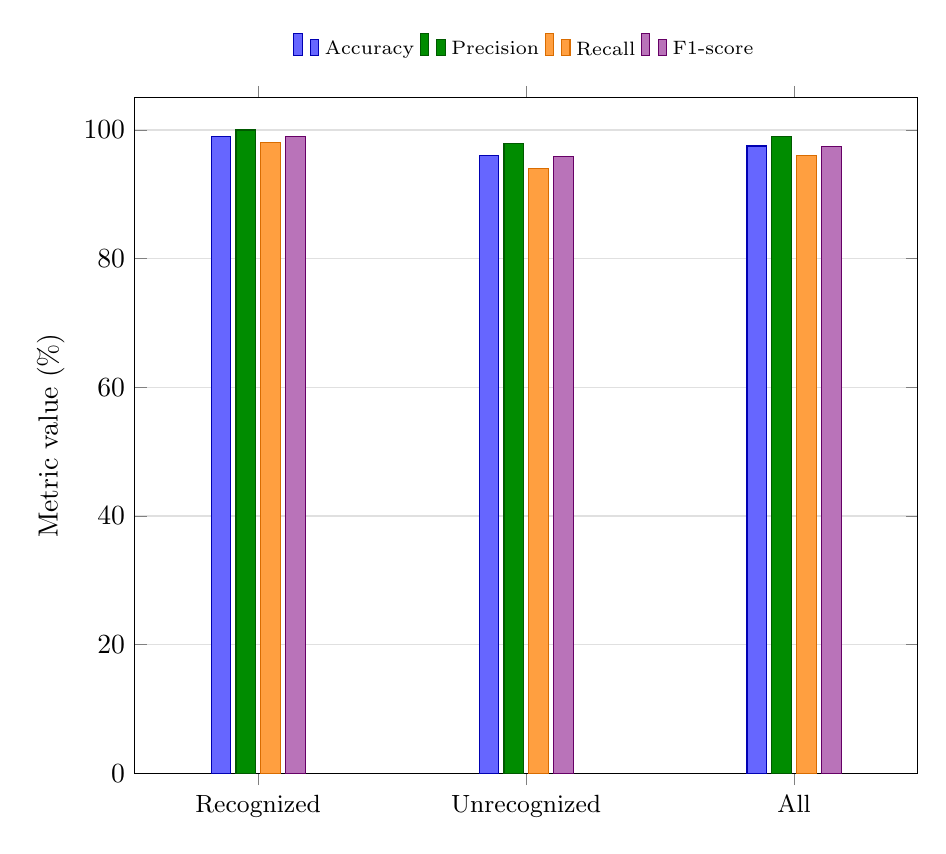
\begin{tikzpicture}
    \begin{axis}[
      ybar,
      width=0.95\textwidth,
      height=4in,
      ymin=0,
      ymax=105,
      ylabel={Metric value (\%)},
      symbolic x coords={Recognized,Unrecognized,All},
      xtick=data,
      x tick label style={font=\small},
      ymajorgrids=true,
      grid style={black!12},
      bar width=7pt,
      enlarge x limits=0.23,
      legend style={font=\scriptsize,at={(0.5,1.04)},anchor=south,legend columns=4,draw=none},
      legend cell align={left}
    ]
      \addplot[fill=blue!60,draw=blue!70!black] coordinates {(Recognized,99.00) (Unrecognized,96.00) (All,97.50)};
      \addplot[fill=green!55!black,draw=green!35!black] coordinates {(Recognized,100.00) (Unrecognized,97.92) (All,98.97)};
      \addplot[fill=orange!75,draw=orange!85!black] coordinates {(Recognized,98.00) (Unrecognized,94.00) (All,96.00)};
      \addplot[fill=violet!55,draw=violet!80!black] coordinates {(Recognized,98.99) (Unrecognized,95.92) (All,97.46)};
      \legend{Accuracy,Precision,Recall,F1-score}
    \end{axis}
  \end{tikzpicture}
  \caption{Trial-level performance metrics by recognized and unrecognized load setup.}
  \label{fig:ch4-group-metrics}
\end{figure}

Table~\ref{tab:ch4-trial-metrics} and Figure~\ref{fig:ch4-group-metrics} show
high overall performance across 200 trial outcomes. Precision is related to
nuisance trips: the 98.97\% overall precision means that only one normal
event was incorrectly tripped in the trial set. Recall is related to safety
sensitivity: the 96.00\% overall recall means that four arc trials were
missed. The recognized-load group had slightly higher recall and no
normal-event false trip, while the unrecognized-load group accounted for
three of the four missed arc trials and the single false trip. This indicates
that the deployed model generalized reasonably, but the unrecognized load
cases remained the more difficult condition.

The trial-level classifier and persistence logic produced balanced
performance: precision remained high for nuisance-trip reduction, while recall
remained high enough to detect most arc trials. These results apply to the
deployed feature contract described in Section~\ref{sec:ch3-feature-contract}:
six selected waveform features were used by the arc model, with context fields
appended to the model vector.

The per-load trial metrics are shown in Table~\ref{tab:ch4-per-load-metrics}.
\begin{table}[H]
  \centering
  \caption{Per-load trial-level performance metrics}
  \label{tab:ch4-per-load-metrics}
  \small
  \setlength{\tabcolsep}{2.5pt}
  \begin{tabular}{p{0.24\textwidth}p{0.15\textwidth}cccc}
    \toprule
    \textbf{Device} & \textbf{Device type} & \textbf{Accuracy} & \textbf{Precision} & \textbf{Recall} & \textbf{F1-score} \\
    \midrule
    Water heater & Resistive & 100\% & 100\% & 100\% & 100\% \\
    Halogen lamp & Resistive & 100\% & 100\% & 100\% & 100\% \\
    Electric kettle & Resistive & 100\% & 100\% & 100\% & 100\% \\
    40W stand fan & Inductive & 100\% & 100\% & 100\% & 100\% \\
    Handheld vacuum & Brushed & 95\% & 100\% & 90\% & 94.74\% \\
    Electrolux vacuum & Brushed & 95\% & 100\% & 90\% & 94.74\% \\
    Angle grinder & Brushed & 95\% & 100\% & 90\% & 94.74\% \\
    Bench cutter & Brushed & 95\% & 100\% & 90\% & 94.74\% \\
    Impact drill & Brushed & 95\% & 90.91\% & 100\% & 95.24\% \\
    Heat gun & Resistive & 100\% & 100\% & 100\% & 100\% \\
    \bottomrule
  \end{tabular}
\end{table}

Table~\ref{tab:ch4-per-load-metrics} shows where the group-level metrics came
from without adding another graph below it. The impact drill is the only load
listed with precision below 100\%, meaning it contributed the normal-event
false trip. The handheld vacuum, vacuum cleaner, angle grinder, and bench
cutter had lower recall, meaning those load cases contributed missed arc
trials.

The same appendix data can also be aggregated by load setup and load family.
For load setup, recognized loads contributed 49 detected arc trials, one
missed arc trial, 50 correct normal trials, and no false trip; unrecognized
loads contributed 47 detected arc trials, three missed arc trials, 49 correct
normal trials, and one false trip. For family grouping, water heater, halogen
lamp, electric kettle, and heat gun were treated as resistive loads; the 40W
stand fan was treated as the inductive load; and the handheld vacuum,
Electrolux vacuum, angle grinder, bench cutter, and impact drill were
treated as brushed or universal-motor loads. These aggregations summarize the
recorded trial tables in Appendix~\ref{app:e}; they are not additional test
conditions.
\begin{figure}[H]
  \centering
  \begin{minipage}{0.47\textwidth}
    \centering
    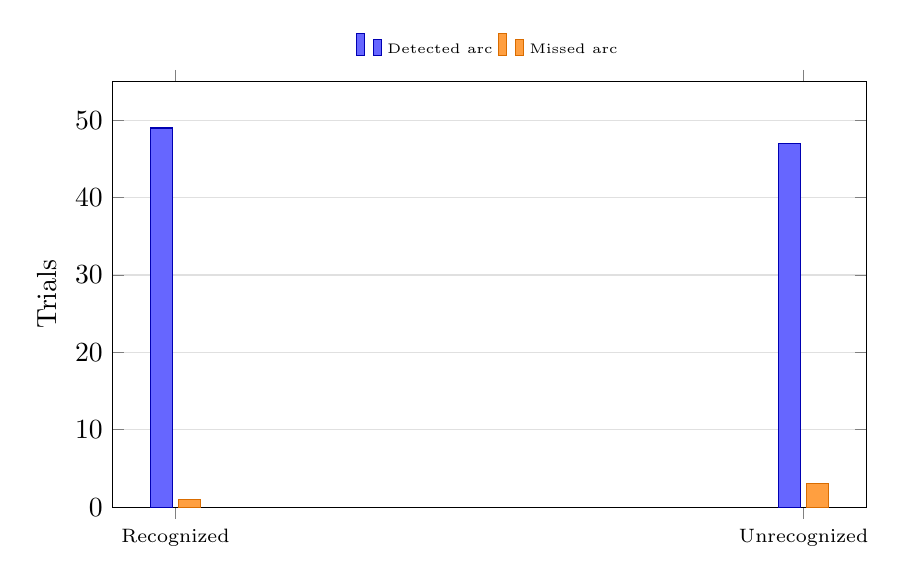
\begin{tikzpicture}
      \begin{axis}[
        ybar,
        width=0.92\linewidth,
        height=2.75in,
        ymin=0,
        ymax=55,
        ylabel={Trials},
        symbolic x coords={Recognized,Unrecognized},
        xtick=data,
        x tick label style={font=\scriptsize},
        ymajorgrids=true,
        grid style={black!12},
        bar width=8pt,
        legend style={font=\tiny,at={(0.5,1.03)},anchor=south,legend columns=2,draw=none},
      ]
        \addplot[fill=blue!60,draw=blue!70!black] coordinates {(Recognized,49) (Unrecognized,47)};
        \addplot[fill=orange!75,draw=orange!85!black] coordinates {(Recognized,1) (Unrecognized,3)};
        \legend{Detected arc,Missed arc}
      \end{axis}
    \end{tikzpicture}
    {\small (a) Arc Trials}
  \end{minipage}\hfill
  \begin{minipage}{0.47\textwidth}
    \centering
    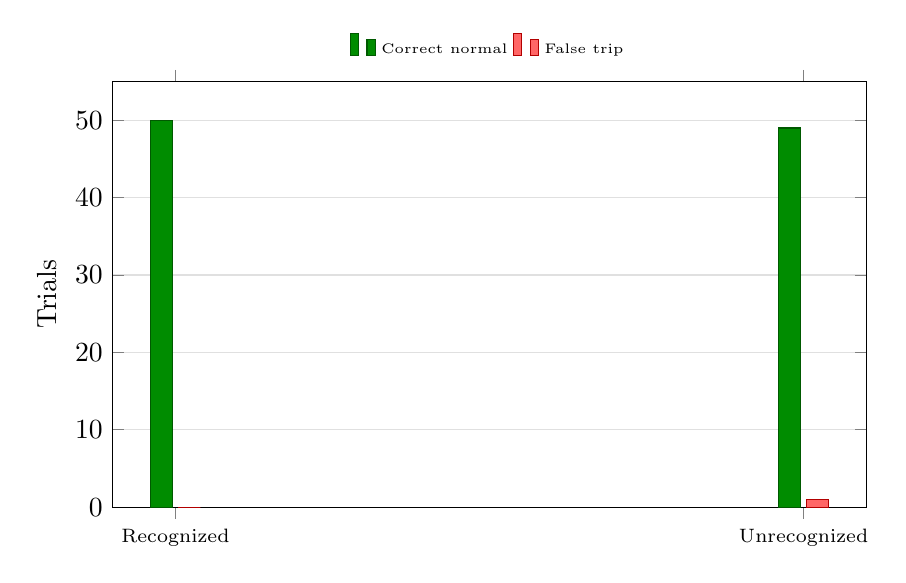
\begin{tikzpicture}
      \begin{axis}[
        ybar,
        width=0.92\linewidth,
        height=2.75in,
        ymin=0,
        ymax=55,
        ylabel={Trials},
        symbolic x coords={Recognized,Unrecognized},
        xtick=data,
        x tick label style={font=\scriptsize},
        ymajorgrids=true,
        grid style={black!12},
        bar width=8pt,
        legend style={font=\tiny,at={(0.5,1.03)},anchor=south,legend columns=2,draw=none},
      ]
        \addplot[fill=green!55!black,draw=green!35!black] coordinates {(Recognized,50) (Unrecognized,49)};
        \addplot[fill=red!60,draw=red!70!black] coordinates {(Recognized,0) (Unrecognized,1)};
        \legend{Correct normal,False trip}
      \end{axis}
    \end{tikzpicture}
    {\small (b) Normal Trials}
  \end{minipage}
  \caption{Grouped trial outcomes for recognized and unrecognized load setups.}
  \label{fig:ch4-setup-outcomes}
\end{figure}

Figure~\ref{fig:ch4-setup-outcomes}(a) shows that the unrecognized group had
more missed arc trials than the recognized group. Figure~\ref{fig:ch4-setup-outcomes}(b)
shows that the only normal-event false trip also came from the unrecognized
group. These results are consistent with the per-load results in
Table~\ref{tab:ch4-per-load-metrics}: generalization loads were still handled
by the protection sequence, but they produced the remaining errors.

\begin{figure}[H]
  \centering
  \begin{minipage}{0.47\textwidth}
    \centering
    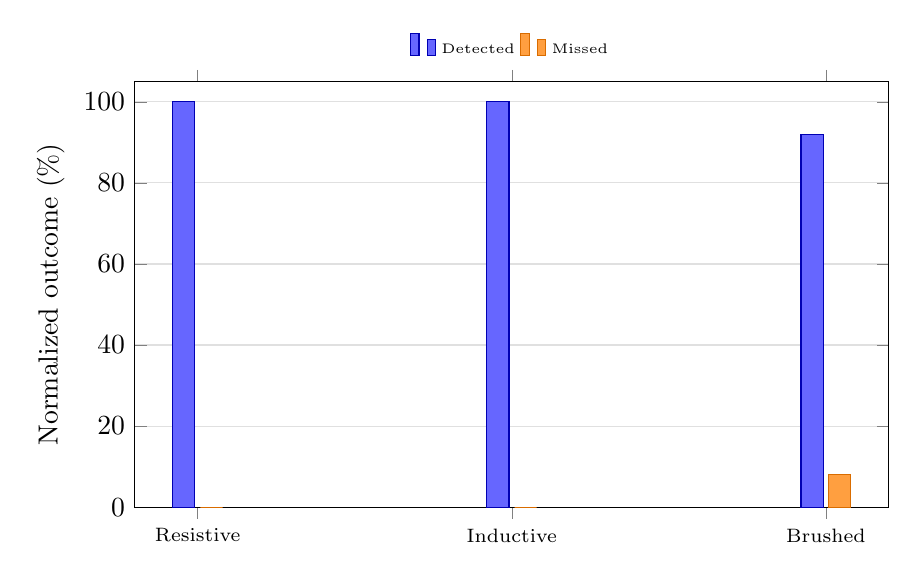
\begin{tikzpicture}
      \begin{axis}[
        ybar,
        width=0.92\linewidth,
        height=2.75in,
        ymin=0,
        ymax=105,
        ylabel={Normalized outcome (\%)},
        symbolic x coords={Resistive,Inductive,Brushed},
        xtick=data,
        x tick label style={font=\scriptsize},
        ymajorgrids=true,
        grid style={black!12},
        bar width=8pt,
        legend style={font=\tiny,at={(0.5,1.03)},anchor=south,legend columns=2,draw=none},
      ]
        \addplot[fill=blue!60,draw=blue!70!black] coordinates {(Resistive,100) (Inductive,100) (Brushed,92)};
        \addplot[fill=orange!75,draw=orange!85!black] coordinates {(Resistive,0) (Inductive,0) (Brushed,8)};
        \legend{Detected,Missed}
      \end{axis}
    \end{tikzpicture}
    {\small (a) Arc Trials}
  \end{minipage}\hfill
  \begin{minipage}{0.47\textwidth}
    \centering
    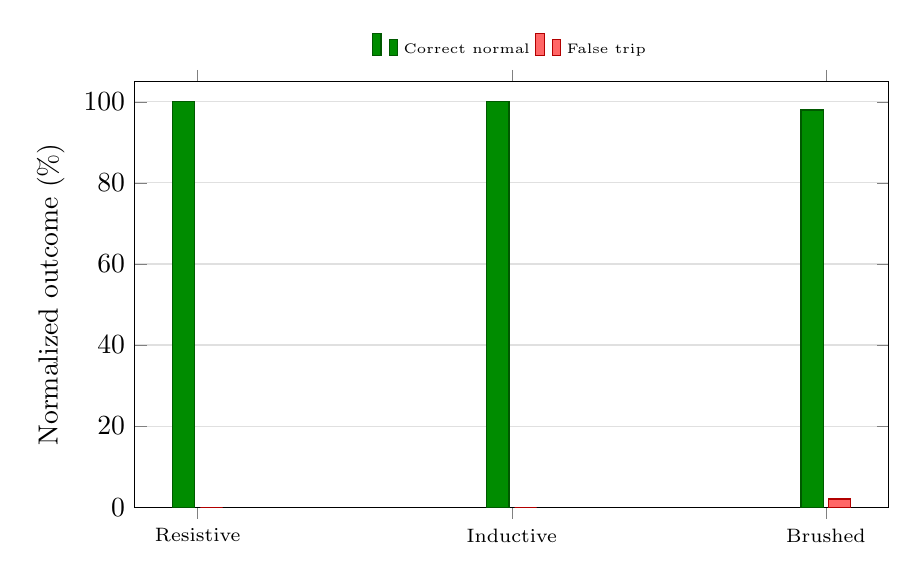
\begin{tikzpicture}
      \begin{axis}[
        ybar,
        width=0.92\linewidth,
        height=2.75in,
        ymin=0,
        ymax=105,
        ylabel={Normalized outcome (\%)},
        symbolic x coords={Resistive,Inductive,Brushed},
        xtick=data,
        x tick label style={font=\scriptsize},
        ymajorgrids=true,
        grid style={black!12},
        bar width=8pt,
        legend style={font=\tiny,at={(0.5,1.03)},anchor=south,legend columns=2,draw=none},
      ]
        \addplot[fill=green!55!black,draw=green!35!black] coordinates {(Resistive,100) (Inductive,100) (Brushed,98)};
        \addplot[fill=red!60,draw=red!70!black] coordinates {(Resistive,0) (Inductive,0) (Brushed,2)};
        \legend{Correct normal,False trip}
      \end{axis}
    \end{tikzpicture}
    {\small (b) Normal Trials}
  \end{minipage}
  \caption{Normalized grouped trial outcomes by load family.}
  \label{fig:ch4-family-outcomes}
\end{figure}

Figure~\ref{fig:ch4-family-outcomes} is normalized because the family groups
did not contain the same number of devices or trials. In
Figure~\ref{fig:ch4-family-outcomes}(a), resistive and inductive load-family
trials had 100\% arc detection, while the brushed-load family had 92\%
arc detection and 8\% missed arc trials. In
Figure~\ref{fig:ch4-family-outcomes}(b), the brushed-load family also
contained the only false trip, giving 98\% correct normal classification and
2\% false-trip outcome for that family. The normalized view therefore shows
that the brushed or universal-motor group was the main source of residual
model error rather than simply the largest group in raw counts.

The exported Random Forest report provides a second view of performance.
The held-out test split contained 10,268 feature rows, including 90 positive
rows. The frame-level confusion matrix contained 10,173 true negatives, 5
false positives, 25 false negatives, and 65 true positives. The corresponding
frame-level accuracy was 99.7078\%, precision was 92.8571\%, recall was
72.2222\%, and F1-score was 81.25\%. At event level, the same report showed
25 true arc events, 21 detected events, 4 missed events, 31 predicted events,
1 false-alarm event, 84.0\% event recall, 96.7742\% event precision, and
89.9358\% event F1-score. The data-preparation, training-report, and
exported-model details supporting these metrics are summarized in
Appendix~\ref{app:f-tinyml-training-summary}.

These model-report values are lower than the final trial-level relay metrics
because they evaluate individual frames and event groupings before the full
trial-level interpretation. This does not invalidate the trial results; it
shows that the firmware's persistence logic is part of the protection
behavior. The deployed model should therefore be judged as a
model-plus-firmware system, not as a standalone frame classifier.

\section{Model Limitations}
\label{sec:ch4-model-limitations}

The main limitation is dataset coverage. The tests included recognized and
unrecognized loads, but they did not cover all appliance families, wiring
conditions, electrode materials, contact gaps, ambient conditions, or utility
waveform variations. The results therefore support prototype feasibility and
future development, but they do not establish compliance with AFCI standards
or replacement equivalence with certified protective devices.

\section{Overall Prototype Feasibility}
\label{sec:ch4-overall-feasibility}

The combined results show that the TinyML Smart Plug achieved the intended
hybrid behavior under controlled laboratory conditions. The calibrated voltage,
current, and temperature measurements were accurate enough to support the
implemented thresholds. The overload tests showed warning behavior followed by
relay trip only when sustained overload persisted. The socket-heating tests
showed that degraded contact can cause faster and more severe heating than
current magnitude alone suggests. The arc-fault tests showed that waveform
features and Random Forest inference can support local relay action for
series-arc events in the tested load set.

The prototype is best interpreted as complementary protection. It adds
socket-level monitoring of overload persistence, thermal rise, and waveform
disturbance, but it is not a replacement for circuit breakers, AFCIs, GFCIs,
proper wiring practice, contact inspection, or certified protection devices.
This boundary matters because the tests were conducted on a laboratory bench,
the thermal estimator was deliberately conservative, and the TinyML model was
trained and evaluated on a finite set of loads and arc conditions.

The results nevertheless support the study objective: a compact
microcontroller-based smart plug can combine calibrated sensing, deterministic
threshold logic, compensated socket-temperature estimation, local TinyML
inference, relay latching, and PWA monitoring in a single prototype. The next
engineering step is not simply to lower thresholds or add more model
complexity; it is to broaden the dataset, validate the thermal estimator
against additional socket constructions, test across more appliance families,
and compare behavior against applicable protection-device standards.

